\chapter{Fyzikální jevy}

Poissonova rovnice umožňuje řešit celou řadu různých fyzikálních jevů. Níže si některé z~nich popíšeme. V~některých případech
je ale nutné fyzikální rovnici napřed upravit na Poissonovu rovnici.

\section{Tepelný tok}

Mějme izotropní tepelně vodivý materiál s~tepelnou vodivostí \(\lambda\). 
Máme-li v materiálu 2 plochy o~obsahu \(S\) ve vzdálenosti \(v\) s~teplotním rozdílem \(\mathrm{d}t\), pak mezi nimi bude proudit tepelný tok 

\begin{equation}
\label{eq:tepelny_tok_1}
P = -\lambda S \frac{\mathrm{d}t}{v}
\end{equation}

Záporné znaménko značí, že směr proudu tepla je opačný než směr růstu
teploty - teplo proudí z~místa s~vyšší teplotou do místa s~nižší teplotou. 

Zapišme tento vztah vektorově. 
Začneme tím, že nahradíme vzdálenost \(v\) vektorem nekonečně malého posunutí \(\mathrm{d}\vect{v}\). Dále podle vztahu \eqref{eq:zmena_pole_gradient} platí \(\mathrm{d}t = \mathrm{t}(x + \mathrm{d}v_x, y + \mathrm{d}v_y, z + \mathrm{d}v_z) - t(x, y, z) = \mathrm{d}\vect{v} \cdot \grad \ \mathrm{t}\):

\begin{equation}
P = -\lambda S \frac{\mathrm{d}\vect{v} \cdot \grad \ \mathrm{t}}{|\mathrm{d}\vect{v}|}
\end{equation}

Vidíme, že \(\frac{\mathrm{d}\vect{v}}{|\mathrm{d}\vect{v}|} = \vect{n}\) je normála plochy \(S\):

\begin{equation}
P = -\lambda \cdot S \cdot \vect{n} \cdot \grad \ \mathrm{t}
\end{equation}

Tepelný tok nekonečně malou plochou \(\mathrm{d}S\) je pak:

\begin{equation}
\mathrm{d}P = -\lambda \cdot \mathrm{d}S \cdot \vect{n} \cdot \grad \ \mathrm{t} = -\lambda \cdot \mathrm{d}\vect{s} \cdot \grad \ \mathrm{t}
\end{equation}

A~celkový tok obecnou plochou \(S\) je pak:

\begin{equation}
P = -\lambda \cdot \int_{S} \grad \ \mathrm{t} \cdot \mathrm{d}\vect{s} 
\end{equation}

Je-li plocha \(S\) uzavřená obklopující těleso \(V\), pak tento výkon musí být roven celkovému výkonu zdroje v~této ploše. Označme hustotu výkonu zdroje \(p_z\). Pak:

\begin{equation}
\int_{V} p_z \mathrm{d}V = -\lambda \cdot \oint_{\partial V} \grad \ \mathrm{t} \cdot \mathrm{d}\vect{s} 
\end{equation} 

Na plošný integrál na pravé straně rovnice použijeme Gaussův teorém: 

\begin{equation}
\int_{V} p_z \mathrm{d}V = -\lambda \cdot \int_{V} \diverg \ \grad \ \mathrm{t} \ \mathrm{d}V = \int_{V} -\lambda \cdot \diverg \ \grad \ \mathrm{t} \ \mathrm{d}V
\end{equation}

Má-li tato rovnice platit pro libovolný objem \(V\), pak musí platit v~každém bodě. Můžeme tedy odstranit objemové integrály:

\begin{equation}
p_z = -\lambda \cdot \diverg \ \grad \ t = -\lambda \cdot \Delta \mathrm{t}
\end{equation}

Tím jsme získaly Poissonovu rovnici pro vedení tepla.

\begin{fact}

\begin{equation}
p_z = -\lambda \cdot \Delta \mathrm{t}
\end{equation}

\begin{equation}
P = -\lambda \cdot \int_{S} \grad \ \mathrm{t} \cdot \mathrm{d}\vect{s} 
\end{equation}

\(P\) - tepelný tok [\(\mathrm{W}\)]

\(p_z\) - hustota tepelného toku z~vnějšího zdroje [\(\mathrm{W} \cdot \mathrm{m}^{-3}\)]

\(t\) - teplota [\(\mathrm{K}, \si{\degree}\mathrm{C}\)]

\(\lambda\) - tepelná vodivost [\(\mathrm{W} \cdot \mathrm{m}^{-1} \cdot \mathrm{K}^{-1}\)] 
\end{fact}

\section{Proud ve vodiči}

Začněme ohmovým zákonem:

\begin{equation}
\label{eq:proud_ve_vodici_1}
I = \frac{U}{R}
\end{equation}

Odpor vodiče o~délce \(l\), průřezu \(S\) a~měrné vodivosti \(sigma\) je určen vztahem \(R = \frac{l}{\sigma S}\). Ten můžeme dosadit do předešlé rovnice. Dále zaveďme elektrický potenciál \(\varphi\). Eletrické napětí \(U\) mezi dvěma body je rovno rozdílu potenciálů v~těchto bodech, tedy \(U = -\mathrm{d}\varphi\). Záporné znaménko značí, že proud teče z~místa s~větším potenciálem do místa s~nižším potenciálem:

\begin{equation}
\label{eq:proud_ve_vodici_2}
I = -\sigma S \frac{-\mathrm{d}\varphi}{l}
\end{equation}

Srovnejme rovnici \eqref{eq:proud_ve_vodici_2} s~rovnicí \eqref{eq:tepelny_tok_1}. Vidíme, že se liší pouze ve veličinách, jinak mají stejnou formu. Proto i~postup jejich řešení bude shodný. Postup proto nebudeme opakovat.

\begin{fact}
\begin{equation}
j_z = -\sigma \cdot \Delta \mathrm{\varphi}
\end{equation}

\begin{equation}
I = -\sigma \cdot \int_{S} \grad \ \mathrm{\varphi} \cdot \mathrm{d}\vect{s} 
\end{equation}

\begin{equation}
U_{AB} = \varphi(A) - \varphi(B) 
\end{equation}

\(I\) - proud [\(\mathrm{A}\)]

\(j_z\) - proudová hustota vnějšího zdroje proudu [\(\mathrm{A} \cdot \mathrm{m}^{-3}\)]

\(\varphi\) - potenciál elektrického pole [\(\mathrm{V}\)]

\(U\) - elektrické napětí [\(\mathrm{V}\)]

\(\sigma\) - elektrická vodivost [\(\mathrm{A} \cdot \mathrm{m}^{-1} \cdot \mathrm{V}^{-1}\)] 
\end{fact}

\section{Elektrostatické pole}

Máme-li dva náboje \(Q_1\) a~\(Q_2\) ve vzdálenosti \(r\) a~v~prostředí s~permitivitou \(\varepsilon\), pak mezi nimi působí síla daná Coulombovým zákonem:

\begin{equation}
\label{eq:coulombuv_zakon}
F = \frac{1}{4 \pi \varepsilon} \cdot \frac{Q_1 \cdot Q_2}{r^2}
\end{equation}

\begin{tikzpicture}
\pgfmathsetmacro{\r}{0.1}
\pgfmathsetmacro{\d}{1.5}
\pgfmathsetmacro{\l}{2}

\draw (-\d, 0) circle[radius=\r];
\draw[->] (-\d - \r, 0) -- (-\d - \l, 0);
\draw (-\d, -\r) node[anchor=north]{\(Q_1\)};
\draw (-\d - \l / 2, 0) node[anchor=north]{\(F\)};

\draw (\d, 0) circle[radius=\r];
\draw[->] (\d + \r, 0) -- (\d + \l, 0);
\draw (\d, -\r) node[anchor=north]{\(Q_2\)};
\draw (\d + \l / 2, 0) node[anchor=north]{\(F\)};
\end{tikzpicture}

Tato síla působí po přímce procházející oběma náboji. Je odpudivá, pokud jsou náboje stejného znaménka a~přitažlivá, pokud jsou opačného znaménka. Kladná síla daná vztahem~\eqref{eq:coulombuv_zakon} je tedy odpudivá. Vztah můžeme přepsat do tvaru 

\begin{equation}
F = \frac{1}{4 \pi \varepsilon} \cdot \frac{Q_1}{r^2} \cdot Q_2 = E \cdot Q_2
\end{equation}

zavedením intenzity elektrického pole

\begin{equation}
\label{eq:intenzita_elektrickeho_pole_bodoveho_naboje}
E = \frac{1}{4 \pi \varepsilon} \cdot \frac{Q_1}{r^2}
\end{equation}

Intenzita elektrického pole tedy určuje sílu vyvolanou nábojem \(Q_1\), která působí na jednotkový náboj \(Q_2\). Síly obecně se vektorově sčítají. Proto se i~intenzity elektrických polí od různých nábojů vektorově sčítají a~vytvářejí celkovou intenzitu. Intenzita elektrického pole je proto vektorovou veličinou.

O~elektrickém poli náboje \(Q_1\) předpokládáme, že existuje nezávisle na náboji \(Q_2\). Protože síla mezi náboji působí vždy po jejich spojnici, tak pro různé polohy náboje \(Q_2\) míří vždy do náboje \(Q_1\). Intenzita elektrického pole \(\vect{E}\) proto vždy míří do nebo z~náboje \(Q_1\), jedná se o~centrální pole.

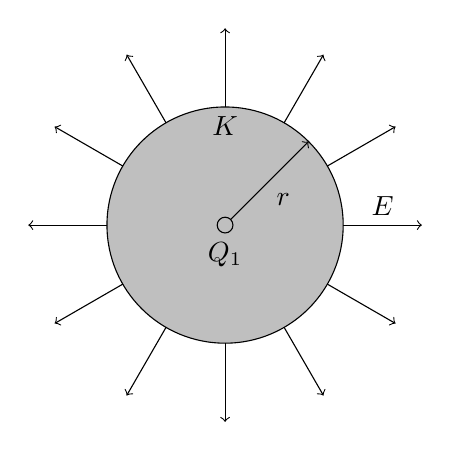
\begin{tikzpicture}
\pgfmathsetmacro{\q}{0.1}
\pgfmathsetmacro{\r}{1.5}
\pgfmathsetmacro{\l}{1}
\pgfmathsetmacro{\n}{12}

\draw[fill=lightgray] (0, 0) circle[radius=\r];

\draw (0, 0) circle[radius=\q];
\draw (0, -\q) node[anchor=north]{\(Q_1\)};

\pgfmathsetmacro{\x}{cos(45)}
\pgfmathsetmacro{\y}{sin(45)}

\draw[->] (\q * \x, \q * \y) -- (\r * \x, \r * \y);
\draw (\r * \x / 2, \r * \y / 2) node[anchor=north west]{\(r\)};

\foreach \alpha in {1, ..., \n} {
	\pgfmathsetmacro{\x}{cos(360 * \alpha / \n)}
	\pgfmathsetmacro{\y}{sin(360 * \alpha / \n)}
	
	\draw[->] (\r * \x, \r * \y) -- (\r * \x + \l * \x, \r * \y + \l * \y);
}

\draw (\r + \l / 2, 0) node[anchor=south]{\(\vect{E}\)};
\draw (0, \r) node[anchor=north]{\(K\)};
\end{tikzpicture}

Zintegrujme vztah~\eqref{eq:intenzita_elektrickeho_pole_bodoveho_naboje} po povrchu \(K\) koule o~poloměru \(r\), v~jejímž středu se nachází náboj \(Q_1\). Intenzita elektrického pole je tedy v~každém bodě kolmá na povrch koule a~má stejnou velikost. Povrch koule se vypočítá podle vztahu \(S = 4 \pi r^2\).

\begin{equation}
\oint_{\partial K} \vect{E} \cdot \mathrm{d}\vect{s} = 4 \pi r^2 \frac{1}{4 \pi \varepsilon} \cdot \frac{Q_1}{r^2} = \frac{Q_1}{\varepsilon}
\end{equation}

Na levou stranu rovnice použijeme Gaussův teorém: 

\begin{equation}
\int_{K} \diverg \vect{E} \cdot \mathrm{d}V = \frac{Q_1}{\varepsilon}
\end{equation}

Povšimněme si, že \(\int_{K} \diverg \vect{E} \cdot \mathrm{d}V\) nezávisí na poloměru koule. Utvoříme-li dvě koule okolo stejného náboje, pak obě budou mít uvedený integrál stejný:

\begin{equation}
\int_{K_1} \diverg \vect{E} \cdot \mathrm{d}V = \int_{K_2} \diverg \vect{E} \cdot \mathrm{d}V
\end{equation}

Předpokládejme, že koule \(K_2\) má větší poloměr než koule \(K_1\). Pro objem mezi oběma koulemi tedy musí platit:

\begin{equation}
\int_{K_2 \setminus K_1} \diverg \vect{E} \cdot \mathrm{d}V = 0
\end{equation}

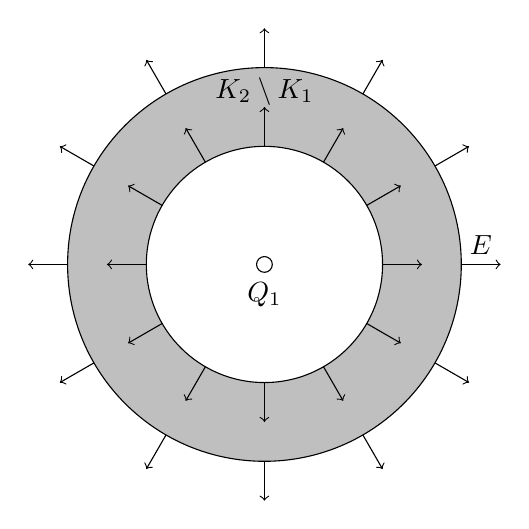
\begin{tikzpicture}
\pgfmathsetmacro{\q}{0.1}
\pgfmathsetmacro{\ra}{1.5}
\pgfmathsetmacro{\rb}{2.5}
\pgfmathsetmacro{\l}{0.5}
\pgfmathsetmacro{\n}{12}

\draw[fill=lightgray] (0, 0) circle[radius=\rb];
\draw[fill=white] (0, 0) circle[radius=\ra];

\draw (0, 0) circle[radius=\q];
\draw (0, -\q) node[anchor=north]{\(Q_1\)};

\foreach \alpha in {1, ..., \n} {
	\pgfmathsetmacro{\x}{cos(360 * \alpha / \n)}
	\pgfmathsetmacro{\y}{sin(360 * \alpha / \n)}
	
	\draw[->] (\ra * \x, \ra * \y) -- (\ra * \x + \l * \x, \ra * \y + \l * \y);
	\draw[->] (\rb * \x, \rb * \y) -- (\rb * \x + \l * \x, \rb * \y + \l * \y);
}

\draw (\rb + \l / 2, 0) node[anchor=south]{\(\vect{E}\)};
\draw (0, \rb) node[anchor=north]{\(K_2 \setminus K_1\)};
\end{tikzpicture}

Nyní si uvědomme, že intenzita elektrického pole \(E\) je symetrická okolo náboje \(Q_1\). Pokud tedy uděláme z~uvedeného objemu mezi koulemi libovolnou výseč, pak musí i~v~tézo výseči být uvecený integrál nulový. Z~takovýchto výsečí je pak možné poskládat libovolné těleso. Můžeme tedy řící, že pro libovolné těleso \(V_0\) které neobsahuje elektrický náboj platí:

\begin{equation}
\int_{V_0} \diverg \vect{E} \cdot \mathrm{d}V = 0
\end{equation}

Libovolné těleso, které obsahuje bodový náboj, pak můžeme zkonstruovat tak, že okolo náboje utvoříme nekonečně malou kouli. Tu pak sjednotíme s~daným tělesem bez této koule. Proto pro libovolné těleso s~bodovým nábojem platí:

\begin{equation}
\begin{split}
\int_{V} \diverg \vect{E} \cdot \mathrm{d}V = \int_{K \cup (V \setminus K)} \diverg \vect{E} \cdot \mathrm{d}V = \\
\int_{K} \diverg \vect{E} \cdot \mathrm{d}V + \int_{V \setminus K} \diverg \vect{E} \cdot \mathrm{d}V = \frac{Q_1}{\varepsilon} + 0 = \frac{Q_1}{\varepsilon}
\end{split}
\end{equation}

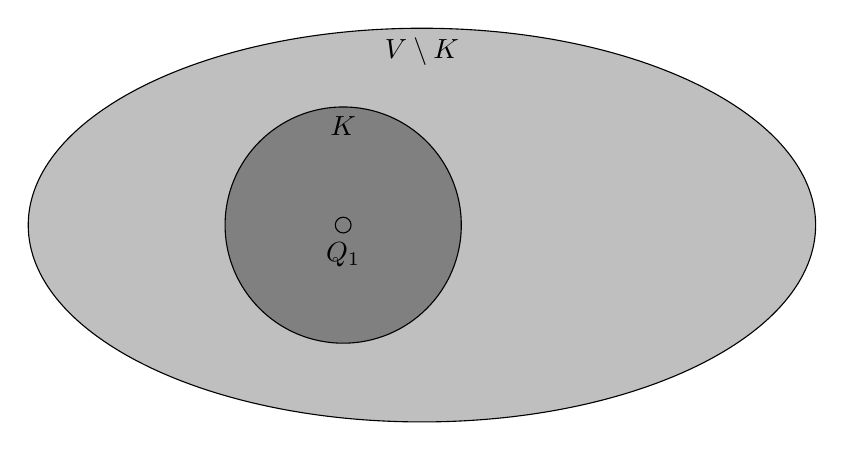
\begin{tikzpicture}
\pgfmathsetmacro{\q}{0.1}
\pgfmathsetmacro{\dx}{1}
\pgfmathsetmacro{\ra}{1.5}
\pgfmathsetmacro{\rb}{2.5}

\draw[fill=lightgray] (\dx, 0) circle[x radius=2*\rb, y radius=\rb];
\draw[fill=gray] (0, 0) circle[radius=\ra];

\draw (0, 0) circle[radius=\q];
\draw (0, -\q) node[anchor=north]{\(Q_1\)};

\draw (0, \ra) node[anchor=north]{\(K\)};
\draw (\dx, \rb) node[anchor=north]{\(V \setminus K\)};
\end{tikzpicture}

Doteď jsme uvažovali pouze jeden bodový náboj \(Q_1\), o~kterém předpokládáme, že je uvnitř tělesa \(V\). Pokud bychom uvnitř tělesa měli více bodových nábojů, pak se jejich intenzity elektrických polí budou sčítat a~bude záležet na celkovém náboji uvnitř tělese: 

\begin{equation}
\int_{V} \diverg \vect{E} \cdot \mathrm{d}V = \frac{1}{\varepsilon} \sum_{i=1}^n Q_i = \frac{Q}{\varepsilon}
\end{equation}

Zaveďme objemovou hustotu náboje \(\rho\) a~proveďme integraci těchto nekokečně malých nábojů přes celé těleso \(V\):

\begin{equation}
\int_{V} \diverg \vect{E} \cdot \mathrm{d}V = \int_{V} \frac{\rho}{\varepsilon} \cdot \mathrm{d}V
\end{equation}

Protože uvedená rovnice platí pro jakékoli těleso \(V\), tak musí platit:

\begin{equation}
\diverg \vect{E} = \frac{\rho}{\varepsilon}
\end{equation}

Podle vztahu \eqref{eq:intenzita_elektrickeho_pole_bodoveho_naboje} závisí intenzita elektrického pole \(\vect{E}\) pouze na vzdálenosti od náboje a~míří z/do náboje. Ve sférickém souřadném systému proto budou splněny podmínky popsané v~\label{sec:potencial_jednoparametrickeho_pole}, inzenzita elektrostatického pole je proto potenciálním polem. Proto můžeme intenzitu elektrického pole vyjádřit ve tvaru 

\begin{equation}
\vect{E} = \grad \ \varphi
\end{equation}

a~získáme tak Poissonovu rovnici

\begin{equation}
\diverg \ \grad \ \varphi = \Delta \varphi = \frac{\rho}{\varepsilon}
\end{equation}

\begin{fact}
\begin{equation}
\Delta \varphi = \frac{\rho}{\varepsilon}
\end{equation}

\begin{equation}
\vect{E} = \grad \ \varphi
\end{equation}

\begin{equation}
U_{AB} = \int_{BA} \vect{E} \cdot \mathrm{d}\vect{l} = \varphi(A) - \varphi(B) 
\end{equation}

\(E\) - intenzita elektrického pole [\(\mathrm{V} \cdot \mathrm{m}^{-1}\)]

\(\varphi\) - potenciál elektrického pole [\(\mathrm{V}\)]

\(U\) - elektrické napětí [\(\mathrm{V}\)]

\(\varepsilon\) - permitivita prostředí [\(\mathrm{F} \cdot \mathrm{m}^{-1}\)]

\(\rho\) - objemová hustota náboje [\(\mathrm{C} \cdot \mathrm{m}^{-3}\)] 
\end{fact}

\section{Gravitační pole}

\section{Stacionární magnetické pole}

Začněme Ampérovým zákonem:

\begin{equation}
\oint_{\partial S} \vect{B} \cdot \mathrm{d}\vect{l} = \mu \cdot I
\end{equation}

Proud \(I\) představuje celkový proud tekoucí uvnitř (libovolné) plochy \(S\), která má hranici \(\partial S\). Neboli, cirkulace vektoru magnetické indukce \(B\) okolo libovolné uzavřené křivky je rovna celkovému proudu, který tato křivka obepíná, násobenému permeabilitou prostředí \(\mu\). Zavedeme proto plošnou hustotu proudu \(j\) a~proud vyjádříme pomocí ní:

\begin{equation}
\oint_{\partial S} \vect{B} \cdot \mathrm{d}\vect{l} = \int_S \mu \cdot \vect{j} \cdot \mathrm{d}\vect{s}
\end{equation}

Na integrál na levé straně rovnice použijeme Stokessovu větu:

\begin{equation}
\int_{S} \rot \ \vect{B} \cdot \mathrm{d}\vect{s} = \int_S \mu \cdot \vect{j} \cdot \mathrm{d}\vect{s}
\end{equation}

Protože plocha \(S\) může být libovolná, tak musí být rovny i~integrované funkce:

\begin{equation}
\rot \ \vect{B} = \mu \cdot \vect{j}
\end{equation}

Touto rovnicí ale není magnetická indukce \(B\) určena jednoznačně. Musíme připojit rovnici udávající, že megnetická indukce je vírové pole. Neexisují tedy zřídla magnetického pole, magnetické monopóly:

\begin{equation}
\diverg \ \vect{B} = 0
\end{equation}

My bychom potřebovali obě rovnice spojit do jedné. Toho můžeme dosáhnout tak, že zavedeme vektorový potenciál \(A\):

\begin{equation}
\vect{B} = \rot \ \vect{A}
\end{equation}

Tím máme zajištěno, že platí

\begin{equation}
\diverg \ \vect{B} = \diverg \ \rot \ \vect{A} = 0
\end{equation}

a~máme tak jedinou rovnici:

\begin{equation}
\rot \ \rot \ \vect{A} = \mu \cdot \vect{j}
\end{equation}

Vektorový potenciál ale není určen jednoznačně. Může proto zavést podmínku 

\begin{equation}
\diverg \ \vect{A} = 0
\end{equation}

Blíže je toto zavedení podmínky popsáno v~sekci~\ref{sec:pole_virova}. Napišme znovu vztah~\eqref{eq:vect_laplace_rozepsany}:

\begin{equation}
\Delta \ \vect{A} = \grad \ \diverg \ \vect{A} - \rot \ \rot \vect{A} 
\end{equation}

Dosazením do pravé strany rovnice získáme vektorovou rovnici, která je v~kartézském souřadném systému řešitelná jako tři nezávislé Poissonovy rovnice pro jednotlivé složky:

\begin{equation}
\Delta \ \vect{A} = -\mu \cdot \vect{j}
\end{equation}

Při studiu elektromagnetické indukce je důležitá veličina magnetického toku plochou. Zaveďme ji tedy.

\begin{equation}
\Phi = \int_S \ \vect{B} \cdot \mathrm{d}\vect{s}
\end{equation}

Prozkoumejme souvislost toku \(\Phi\) s~vektorovým potenciálem \(A\). V~rovnici pomocí něj vyjádříme magnetickou indukci a~použijeme Stokessovu větu:

\begin{equation}
\Phi = \int_S \ \rot \ \vect{A} \cdot \mathrm{d}\vect{s} = \oint_{\partial S} \vect{A} \cdot \mathrm{d}\vect{l}
\end{equation}

\begin{fact}
\begin{equation}
\Delta \ \vect{A} = -\mu \cdot \vect{j}
\end{equation}

\begin{equation}
\vect{B} = \rot \ \vect{A}
\end{equation}

\begin{equation}
\Phi = \oint_{\partial S} \vect{A} \cdot \mathrm{d}\vect{l}
\end{equation}

\(j\) - proudová hustota [\(\mathrm{A} \cdot \mathrm{m}^{-3}\)]

\(\mu\) - permeabilita prostředí [\(\mathrm{H} \cdot \mathrm{m}^{-1}\)]

\(\vect{A}\) - vektorový potenciál magnetického pole [\(\mathrm{T} \cdot \mathrm{m}\)]

\(\vect{B}\) - magnetická indukce [\(\mathrm{T}\)]

\(\Phi\) - magnetický tok [\(\mathrm{Wb}\)]
\end{fact}
